\clearpage
\VerdierPhysicalPageAnchor{0083}%
\VerdierSemanticAnchor{ch1-3-1-1-additivity}
The category $\operatorname{tr}_1(C)$ is additive. The direct sum of
$X\xrightarrow{f}Y$ and $X'\xrightarrow{f'}Y'$ is:

\VerdierSemanticAnchor{ch1-3-1-1-direct-sum}
\begin{equation*}
  X\oplus X'
  \xrightarrow{\left(\begin{smallmatrix}f&0\\0&f'\end{smallmatrix}\right)}
  Y\oplus Y'.
\end{equation*}

\VerdierSemanticAnchor{ch1-3-1-2}
\noindent\textbf{3.1.2.}\quad
Let $X\xrightarrow{f}Y$ be an object of $\operatorname{tr}_1(C)$. Set:

\VerdierSemanticAnchor{ch1-3-1-2-cone-object}
\begin{equation*}
  c(f)^i=Y^i\oplus X^{i+1},
\end{equation*}

\VerdierSemanticAnchor{ch1-3-1-2-eq1}
\begin{equation}
  d_{c(f)}^i=
  \begin{pmatrix}
    d_Y^i & f^{i+1}\\
    0 & -d_X^{i+1}
  \end{pmatrix}
  \colon Y^i\oplus X^{i+1}\longrightarrow Y^{i+1}\oplus X^{i+2}.
  \tag{3.1.2.1}
\end{equation}

\VerdierSemanticAnchor{ch1-3-1-2-cone-verification}
One checks that a complex of objects of $C$ has thereby been defined.
\VerdierSemanticAnchor{ch1-3-1-2-cone-name}
This complex is denoted by $c(f)$ and is called the \emph{cone of the morphism}
$f$. Now let:

\VerdierSemanticAnchor{ch1-3-1-2-morphism-setup}
\begin{equation*}
  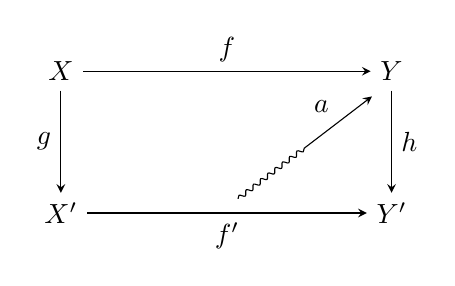
\begin{tikzpicture}[>=stealth,baseline=(current bounding box.center)]
    \node (X)  at (0,1.8) {$X$};
    \node (Y)  at (4.2,1.8) {$Y$};
    \node (Xp) at (0,0) {$X'$};
    \node (Yp) at (4.2,0) {$Y'$};
    \draw[->] (X) -- node[above] {$f$} (Y);
    \draw[->] (X) -- node[left] {$g$} (Xp);
    \draw[->] (Y) -- node[right] {$h$} (Yp);
    \draw[->] (Xp) -- node[below] {$f'$} (Yp);
    \draw[decorate,decoration={snake,amplitude=0.8pt,segment length=3.3pt}]
      (2.25,0.18) -- (3.10,0.83);
    \draw[->] (3.10,0.83) -- node[above left] {$a$} (3.95,1.48);
  \end{tikzpicture}
\end{equation*}
be a morphism of $\operatorname{tr}_1(C)$. Set:

\VerdierSemanticAnchor{ch1-3-1-2-eq2}
\begin{equation}
  c((g,h,a))^i=
  \begin{pmatrix}
    h^i & a^i\\
    0 & g^{i+1}
  \end{pmatrix}
  \colon Y^i\oplus X^{i+1}\longrightarrow Y'^i\oplus X'^{i+1}.
  \tag{3.1.2.2}
\end{equation}

\VerdierSemanticAnchor{ch1-3-1-2-complex-morphism}
These morphisms commute with the differentials of $c(f)$ and $c(f')$ and
consequently define a morphism of complexes:

\VerdierSemanticAnchor{ch1-3-1-2-eq3}
\begin{equation}
  c((g,h,a))\colon c(f)\longrightarrow c(f').
  \tag{3.1.2.3}
\end{equation}

\VerdierSemanticAnchor{ch1-3-1-2-cone-functor}
One checks that in this way a functor
$c\colon\operatorname{tr}_1(C)\longrightarrow\operatorname{comp}(C)$
has been defined, called the \emph{cone functor}.

\VerdierSemanticAnchor{ch1-3-1-2-s-functor}
Denote by
$s\colon\operatorname{comp}(C)\longrightarrow\operatorname{tr}_1(C)$
the functor $X\longmapsto(0\longrightarrow X)$.
\VerdierSemanticAnchor{ch1-3-1-2-phi-setup}
For every object $X\xrightarrow{f}Y$ of $\operatorname{tr}_1(C)$, denote by
$\Phi(f)\colon(X\xrightarrow{f}Y)\longrightarrow s c(f)$ the
